Voor ons eindwerk kregen we een Dell PowerEdge 2950 om onze virtualisatie in te runnen. Deze server hebben wij volledig geconfigureerd.

De eerste problemen onstonden al na enkele minuten. Deze server kon namelijk niet booten vanaf een USB, dit terwijl er wel degelijk 4 poorten aanwezig waren. Hierna hebben we Debian Wheezy\cite{wheezy} ge\"installeerd met behulp van een bootable CD. Deze installatie verliep zonder verdere problemen.

Na de installatie hebben wij de repositories van OpenVZ\cite{openvz} toegevoegd aan de \texttt{sources.list} en OpenVZ ge\"installeerd.
Ook deze installatie verliep van een leie dakje.

Hierna hebben wij een IP-adres range gekozen voor de verschillende services die moeten draaien op deze server. OpenVZ biedt ons de mogelijkheid verschillende containers\cite{openvzcontainers} te maken die bovenop deze OpenVZ omgeving draaien. Elke service krijgt daarom een eigen container met Debian Wheezy, behalve de container die instaat voor de controle van de ``Memory-based'' oefeningen. Deze service draait  onder Ubuntu 7.10\cite{openvzubuntu}.

De keuze voor Ubuntu 7.10 is enkel en alleen omwille van de gcc\cite{gcc} versie (gcc-3.3). Deze gcc-versie houdt nog geen rekening met stack-protection waardoor onze exploit-oefeningen juist gaan functioneren.

\subsection{Host (129)}
Dit is het hostsysteem op onze server. Hierop hebben we OpenVZ ge\"installeerd zodat we containers kunnen runnen. We hebben ook enkele scripts ge\"installeerd zodat de Coderunner kan \emph{praten} met de host om containers op te starten en af te zetten.

\subsection{Website (130)}
Deze container draait Debian Wheezy.\\
Apache2\cite{apache} werd hier ge\"installeerd.

Door middel van crontab zal het script ``/root/sync\_website.sh'' elke minuut gaan controleren of er een nieuwe git commit is geweest. Een positieve git commit wijst op een lokale aanpassing van de website. Deze lokale aanpassing zal door het script worden overgenomen worden in \texttt{/var/www}. Hierdoor zal de webserver bijna onmiddellijk gesynchroniseerd worden met de lokale website versie.

Een tweede script (/root/sync\_oef.php), dat opgeroepen wordt in het sync\_website.sh script, zal ervoor zorgen dat iedere gebruiker het juiste aantal oefeningen in zijn/haar persoonlijk overzicht heeft staan.

De website is opgebouwd aan de hand van het framework van het vak ``Dynamische Websites''. We hebben voor dit framework gekozen omdat het hierdoor makkelijk is om nieuwe zaken te integreren en de site te beveiligen.

Voor het design van de site hebben we onze eigen CSS geschreven en geprobeerd om deze responsive te maken zodat, indien de website ooit online komt te staan, deze ook op tablets zal functioneren.

De site is onderverdeeld in vier delen: Oefeningen, Exploits, Downloadables en links.

Bij oefeningen kunnen de gebruikers kiezen tussen enkele categorie\"en:
\begin{itemize}
\item Web-based: bevat oefeningen waar de gebruiker de browser moet hacken. Dit zijn oefeningen op SQL injection, cookie tampering, XSS, \ldots
\item Memory based: bestaat uit verschillende bufferoverflow oefeningen die gecontroleerd worden aan de hand van openVZ containers.
\item Forensics: de gebruiker moet in deze categorie wachtwoorden terug vinden die op verschillende manieren verborgen zijn.
\item Encryptie: bevat oefeningen waarbij de gebruiker wachtwoorden die op verschillende manieren versleuteld zijn moet decrypteren.
\item Trivia: deze categorie bestaat uit vragenreeksen van 10 vragen. Het grootste deel van de vragen komt uit de examenwiki zodat de studenten ook de theoretische kant goed kunnen inoefenen.
\item Capture the flag: deze categorie bevat capture the flag oefeningen waarbij de gebruiker bepaalde opdrachten moet voltooien.
\item Complex: hierin bevinden zich oefeningen die een combinatie zijn van oefeningen uit de andere categorie\"en. Deze oefeningen staan op apparte sites en bevinden zich dus niet meer in het framework vermits ze hierdoor veel meer vrijheden hebben, wat noodzakelijk was.
\end{itemize}

Exploits bevat enkele tutorials en ook een demo formulier voor e-mailspoofing.

Downloadables bevat downloadbare omgevingen/oefeningen die de gebruiker op zijn computer kan oplossen.

In Links staan enkele andere CTF sites en andere nuttige sites in verband met beveiliging.

Verder bevindt zich op de site een highscore pagina, een overzicht van de gemaakte oefeningen met achievements, een registratie pagina, een verborgen konami pagina, een speciale error pagina en een settings pagina.
\subsection{SQL (131)}
Deze container draait Debian Wheezy.\\
MySQL werd hier ge\"installeerd.

De keuze om de website en de SQL-server in een aparte container te draaien is om de veiligheid van beide containers te garanderen.

De database bestaat uit twee verschillende schema’s:
\begin{figure}[H]
\centering
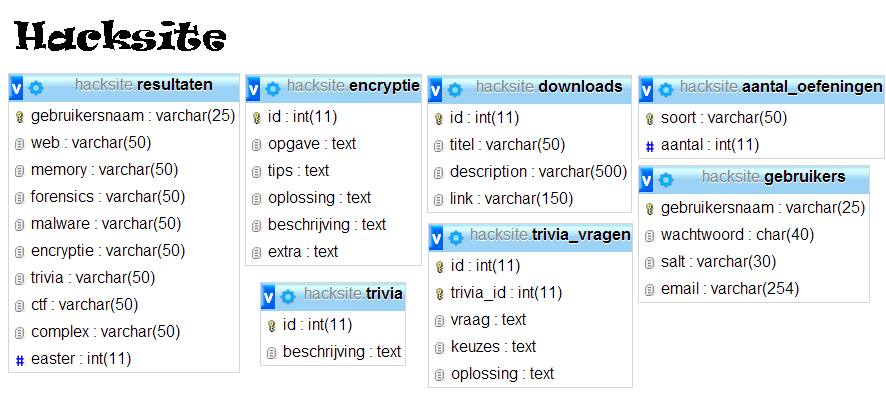
\includegraphics[scale=0.5]{systeem/db1.jpg}
\end{figure}
	\begin{itemize}
	\item aantal\_oefeningen: bevat het aantal oefeningen dat elke soort heeft. Hierdoor krijgen de gebruikers een achievement als ze alle oefeningen van een categorie hebben opgelost en wordt het totaal aantal oefeningen berekend, \ldots
	\item downloads: hierin bevinden de downloadbare bestanden zich zodat deze automatisch uitgelezen kunnen worden.
	\item Encryptie: in deze tabel worden de encryptie oefeningen bewaard. Hierdoor kunnen deze makkelijk toegevoegd worden.
	\item Gebruikers: hierin staan alle users met een sha1 gehasht en gesalt paswoord zodat de wachtwoorden vrij veilig zijn.
	\item Resultaten: hierin staat voor elke gebruiker bij elke oefeningensoort een string. Deze string bevat `j', `n' en `-'. Indien er een `j' staat heeft de gebruiker de oefening opgelost, bij een `n' nog niet. Wanneer er een - staat heeft de categorie nog niet zoveel oefeningen en kan dit `-' dus gereplaced worden met een `j' of een `n' wanneer deze wel bestaat. We hebben hiervoor gekozen omdat na de controle van de bufferoverflow oefening in de openVZ container met \'e\'en regex de feedback toegevoegd kan worden aan de database.
	\item trivia: hierin staan alle vragenreeksen zodat de vragen mooi per 10 verdeeld worden.
	\item Trivia\_vragen: hierin staan alle quiz vragen en de oefeningen reeks waarbij ze behoren.
	\end{itemize}
\begin{figure}[H]
\centering
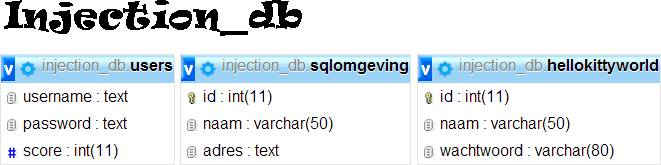
\includegraphics[scale=0.5]{systeem/db2.jpg}
\end{figure}
	\begin{itemize}
	\item hellokittyworld: deze tabel wordt gebruikt voor SQL injection bij de vierde complexe oefening.
	\item Sqlomgeving: deze tabel wordt gebruikt voor SQL injection bij de vierde complexe oefening.
	\item Users: deze tabel wordt gebruikt voor SQL injection bij enkele web-based oefeningen en bij de tweede complexe oefening.
	\end{itemize}


\subsection{Coderunner (132)}
Hierop draait een Perl script die instaat voor het runnen van de memory-based oefeningen. De website connecteert op een poort (12345) waar dit script op draait. Bij het verzenden van een oefening op de website, stuurt een PHP script deze code door naar de Coderunner. De Coderunner connecteert dan op zijn beurt met het hostsysteem om een nieuwe container op te starten. Van zodra deze is opgestart, connecteert de Coderunner met de nieuwe container en wordt de code uitgevoerd op deze container. Het resultaat wordt ge\"interpreteerd door de Coderunner en wordt daarna opgeslagen in de database van de Website zodat de gebruiker kan zien of hij/zij de oefening juist had. Als laatste stuurt de Coderunner een bericht naar het hostsysteem om de Container te verwijderen.
